\documentclass[ignorenonframetext,]{beamer}
\setbeamertemplate{caption}[numbered]
\setbeamertemplate{caption label separator}{: }
\setbeamercolor{caption name}{fg=normal text.fg}
\beamertemplatenavigationsymbolsempty
\usepackage{lmodern}
\usepackage{amssymb,amsmath}
\usepackage{ifxetex,ifluatex}
\usepackage{fixltx2e} % provides \textsubscript
\ifnum 0\ifxetex 1\fi\ifluatex 1\fi=0 % if pdftex
  \usepackage[T1]{fontenc}
  \usepackage[utf8]{inputenc}
\else % if luatex or xelatex
  \ifxetex
    \usepackage{mathspec}
  \else
    \usepackage{fontspec}
  \fi
  \defaultfontfeatures{Ligatures=TeX,Scale=MatchLowercase}
\fi
\usecolortheme{crane}
\usefonttheme{structurebold}
% use upquote if available, for straight quotes in verbatim environments
\IfFileExists{upquote.sty}{\usepackage{upquote}}{}
% use microtype if available
\IfFileExists{microtype.sty}{%
\usepackage{microtype}
\UseMicrotypeSet[protrusion]{basicmath} % disable protrusion for tt fonts
}{}
\newif\ifbibliography
\hypersetup{
            pdftitle={How Much Money Can You Make},
            pdfauthor={Heming and Kit Nga Chou},
            pdfborder={0 0 0},
            breaklinks=true}
\urlstyle{same}  % don't use monospace font for urls
\usepackage{color}
\usepackage{fancyvrb}
\newcommand{\VerbBar}{|}
\newcommand{\VERB}{\Verb[commandchars=\\\{\}]}
\DefineVerbatimEnvironment{Highlighting}{Verbatim}{commandchars=\\\{\}}
% Add ',fontsize=\small' for more characters per line
\usepackage{framed}
\definecolor{shadecolor}{RGB}{248,248,248}
\newenvironment{Shaded}{\begin{snugshade}}{\end{snugshade}}
\newcommand{\KeywordTok}[1]{\textcolor[rgb]{0.13,0.29,0.53}{\textbf{#1}}}
\newcommand{\DataTypeTok}[1]{\textcolor[rgb]{0.13,0.29,0.53}{#1}}
\newcommand{\DecValTok}[1]{\textcolor[rgb]{0.00,0.00,0.81}{#1}}
\newcommand{\BaseNTok}[1]{\textcolor[rgb]{0.00,0.00,0.81}{#1}}
\newcommand{\FloatTok}[1]{\textcolor[rgb]{0.00,0.00,0.81}{#1}}
\newcommand{\ConstantTok}[1]{\textcolor[rgb]{0.00,0.00,0.00}{#1}}
\newcommand{\CharTok}[1]{\textcolor[rgb]{0.31,0.60,0.02}{#1}}
\newcommand{\SpecialCharTok}[1]{\textcolor[rgb]{0.00,0.00,0.00}{#1}}
\newcommand{\StringTok}[1]{\textcolor[rgb]{0.31,0.60,0.02}{#1}}
\newcommand{\VerbatimStringTok}[1]{\textcolor[rgb]{0.31,0.60,0.02}{#1}}
\newcommand{\SpecialStringTok}[1]{\textcolor[rgb]{0.31,0.60,0.02}{#1}}
\newcommand{\ImportTok}[1]{#1}
\newcommand{\CommentTok}[1]{\textcolor[rgb]{0.56,0.35,0.01}{\textit{#1}}}
\newcommand{\DocumentationTok}[1]{\textcolor[rgb]{0.56,0.35,0.01}{\textbf{\textit{#1}}}}
\newcommand{\AnnotationTok}[1]{\textcolor[rgb]{0.56,0.35,0.01}{\textbf{\textit{#1}}}}
\newcommand{\CommentVarTok}[1]{\textcolor[rgb]{0.56,0.35,0.01}{\textbf{\textit{#1}}}}
\newcommand{\OtherTok}[1]{\textcolor[rgb]{0.56,0.35,0.01}{#1}}
\newcommand{\FunctionTok}[1]{\textcolor[rgb]{0.00,0.00,0.00}{#1}}
\newcommand{\VariableTok}[1]{\textcolor[rgb]{0.00,0.00,0.00}{#1}}
\newcommand{\ControlFlowTok}[1]{\textcolor[rgb]{0.13,0.29,0.53}{\textbf{#1}}}
\newcommand{\OperatorTok}[1]{\textcolor[rgb]{0.81,0.36,0.00}{\textbf{#1}}}
\newcommand{\BuiltInTok}[1]{#1}
\newcommand{\ExtensionTok}[1]{#1}
\newcommand{\PreprocessorTok}[1]{\textcolor[rgb]{0.56,0.35,0.01}{\textit{#1}}}
\newcommand{\AttributeTok}[1]{\textcolor[rgb]{0.77,0.63,0.00}{#1}}
\newcommand{\RegionMarkerTok}[1]{#1}
\newcommand{\InformationTok}[1]{\textcolor[rgb]{0.56,0.35,0.01}{\textbf{\textit{#1}}}}
\newcommand{\WarningTok}[1]{\textcolor[rgb]{0.56,0.35,0.01}{\textbf{\textit{#1}}}}
\newcommand{\AlertTok}[1]{\textcolor[rgb]{0.94,0.16,0.16}{#1}}
\newcommand{\ErrorTok}[1]{\textcolor[rgb]{0.64,0.00,0.00}{\textbf{#1}}}
\newcommand{\NormalTok}[1]{#1}
\usepackage{graphicx,grffile}
\makeatletter
\def\maxwidth{\ifdim\Gin@nat@width>\linewidth\linewidth\else\Gin@nat@width\fi}
\def\maxheight{\ifdim\Gin@nat@height>\textheight0.8\textheight\else\Gin@nat@height\fi}
\makeatother
% Scale images if necessary, so that they will not overflow the page
% margins by default, and it is still possible to overwrite the defaults
% using explicit options in \includegraphics[width, height, ...]{}
\setkeys{Gin}{width=\maxwidth,height=\maxheight,keepaspectratio}

% Prevent slide breaks in the middle of a paragraph:
\widowpenalties 1 10000
\raggedbottom

\AtBeginPart{
  \let\insertpartnumber\relax
  \let\partname\relax
  \frame{\partpage}
}
\AtBeginSection{
  \ifbibliography
  \else
    \let\insertsectionnumber\relax
    \let\sectionname\relax
    \frame{\sectionpage}
  \fi
}
\AtBeginSubsection{
  \let\insertsubsectionnumber\relax
  \let\subsectionname\relax
  \frame{\subsectionpage}
}

\setlength{\parindent}{0pt}
\setlength{\parskip}{6pt plus 2pt minus 1pt}
\setlength{\emergencystretch}{3em}  % prevent overfull lines
\providecommand{\tightlist}{%
  \setlength{\itemsep}{0pt}\setlength{\parskip}{0pt}}
\setcounter{secnumdepth}{0}

\title{How Much Money Can You Make}
\author{Heming and Kit Nga Chou}
\date{Winter 2019}

\begin{document}
\frame{\titlepage}

\begin{frame}[fragile]

\begin{block}{INTRO}

We are interested in how much money do professors make, and what affects
the salary distribution. Used data from:
``\url{https://vincentarelbundock.github.io/Rdatasets/datasets.html}''

\begin{Shaded}
\begin{Highlighting}[]
\NormalTok{prof_salary <-}
\StringTok{  }\NormalTok{readr}\OperatorTok{::}\KeywordTok{read_csv}\NormalTok{(}\StringTok{"salaries_prof.csv"}\NormalTok{)}
\end{Highlighting}
\end{Shaded}

\begin{verbatim}
## Warning: Missing column names filled in: 'X1' [1]
\end{verbatim}

\begin{verbatim}
## Parsed with column specification:
## cols(
##   X1 = col_double(),
##   rank = col_character(),
##   discipline = col_character(),
##   yrs.since.phd = col_double(),
##   yrs.service = col_double(),
##   sex = col_character(),
##   salary = col_double()
## )
\end{verbatim}

\end{block}

\end{frame}

\begin{frame}[fragile]{PACKAGES}

We used the following libraries:

\begin{Shaded}
\begin{Highlighting}[]
\KeywordTok{library}\NormalTok{(tidyverse)}
\KeywordTok{library}\NormalTok{(dplyr)}
\end{Highlighting}
\end{Shaded}

\begin{Shaded}
\begin{Highlighting}[]
\KeywordTok{library}\NormalTok{(}\StringTok{"RColorBrewer"}\NormalTok{)}
\KeywordTok{library}\NormalTok{(}\StringTok{"paletteer"}\NormalTok{)}
\end{Highlighting}
\end{Shaded}

\begin{block}{HAVE A LOOK}

\begin{Shaded}
\begin{Highlighting}[]
\NormalTok{prof_salary }\OperatorTok\StringTok{ }
\StringTok{  }\NormalTok{skimr}\OperatorTok{::}\KeywordTok{skim}\NormalTok{()}
\end{Highlighting}
\end{Shaded}

\begin{verbatim}
## Skim summary statistics
##  n obs: 397 
##  n variables: 7 
## 
## -- Variable type:character -----------------------------------------------------
##    variable missing complete   n min max empty n_unique
##  discipline       0      397 397   1   1     0        2
##        rank       0      397 397   4   9     0        3
##         sex       0      397 397   4   6     0        2
## 
## -- Variable type:numeric -------------------------------------------------------
##       variable missing complete   n      mean       sd    p0   p25    p50
##         salary       0      397 397 113706.46 30289.04 57800 91000 107300
##             X1       0      397 397    199      114.75     1   100    199
##    yrs.service       0      397 397     17.61    13.01     0     7     16
##  yrs.since.phd       0      397 397     22.31    12.89     1    12     21
##     p75   p100     hist
##  134185 231545 ▃▇▇▅▃▂▁▁
##     298    397 ▇▇▇▇▇▇▇▇
##      27     60 ▇▆▅▅▂▂▁▁
##      32     56 ▆▇▇▇▆▅▂▁
\end{verbatim}

\end{block}

\begin{block}{QUESTIONS?}

\begin{enumerate}
\def\labelenumi{\arabic{enumi}.}
\tightlist
\item
  Who makes the most money?
\item
  How does salary differ by ranks?
\item
  Does salary differ by gender?
\item
  What is discipline?
\item
  Does the amount of time you spent on the job affect your income?
\end{enumerate}

\begin{Shaded}
\begin{Highlighting}[]
\NormalTok{knitr}\OperatorTok{::}\KeywordTok{include_graphics}\NormalTok{(}\StringTok{"profledford.jpg"}\NormalTok{)}
\end{Highlighting}
\end{Shaded}

\begin{center}
\includegraphics[width=0.3\linewidth]{profledford} \end{center}

\end{block}

\begin{block}{MAKE TIDY DATA}

\begin{Shaded}
\begin{Highlighting}[]
\NormalTok{prof_salary_tidy <-prof_salary }\OperatorTok\StringTok{ }
\StringTok{  }\NormalTok{dplyr}\OperatorTok{::}\KeywordTok{rename}\NormalTok{(}
    \DataTypeTok{Participants =}\NormalTok{ X1,}
    \DataTypeTok{Rank =}\NormalTok{ rank,}
    \DataTypeTok{Discipline =}\NormalTok{ discipline,}
    \DataTypeTok{Yrs_since_PhD =}\NormalTok{ yrs.since.phd,}
    \DataTypeTok{Yrs_service =}\NormalTok{ yrs.service,}
    \DataTypeTok{Sex =}\NormalTok{ sex,}
    \DataTypeTok{Salary =}\NormalTok{ salary)}
\NormalTok{prof_salary_tidy}
\end{Highlighting}
\end{Shaded}

\begin{verbatim}
## # A tibble: 397 x 7
##    Participants Rank      Discipline Yrs_since_PhD Yrs_service Sex   Salary
##           <dbl> <chr>     <chr>              <dbl>       <dbl> <chr>  <dbl>
##  1            1 Prof      B                     19          18 Male  139750
##  2            2 Prof      B                     20          16 Male  173200
##  3            3 AsstProf  B                      4           3 Male   79750
##  4            4 Prof      B                     45          39 Male  115000
##  5            5 Prof      B                     40          41 Male  141500
##  6            6 AssocProf B                      6           6 Male   97000
##  7            7 Prof      B                     30          23 Male  175000
##  8            8 Prof      B                     45          45 Male  147765
##  9            9 Prof      B                     21          20 Male  119250
## 10           10 Prof      B                     18          18 Fema~ 129000
## # ... with 387 more rows
\end{verbatim}

\end{block}

\begin{block}{OVERALL DISTRIBUTION}

\begin{Shaded}
\begin{Highlighting}[]
\NormalTok{prof_salary_tidy }\OperatorTok\StringTok{ }
\StringTok{  }\KeywordTok{ggplot}\NormalTok{(}\KeywordTok{aes}\NormalTok{(}\DataTypeTok{x=}\NormalTok{Salary))}\OperatorTok{+}
\StringTok{  }\KeywordTok{geom_histogram}\NormalTok{(}\KeywordTok{aes}\NormalTok{(}\DataTypeTok{y =}\NormalTok{ ..density..), }\DataTypeTok{fill=}\StringTok{"darkgreen"}\NormalTok{, }\DataTypeTok{alpha=}\FloatTok{0.8}\NormalTok{, }\DataTypeTok{color=}\StringTok{"black"}\NormalTok{)}\OperatorTok{+}
\StringTok{  }\KeywordTok{geom_density}\NormalTok{(}\DataTypeTok{color=}\StringTok{"orange"}\NormalTok{)}
\end{Highlighting}
\end{Shaded}

\begin{verbatim}
## `stat_bin()` using `bins = 30`. Pick better value with `binwidth`.
\end{verbatim}

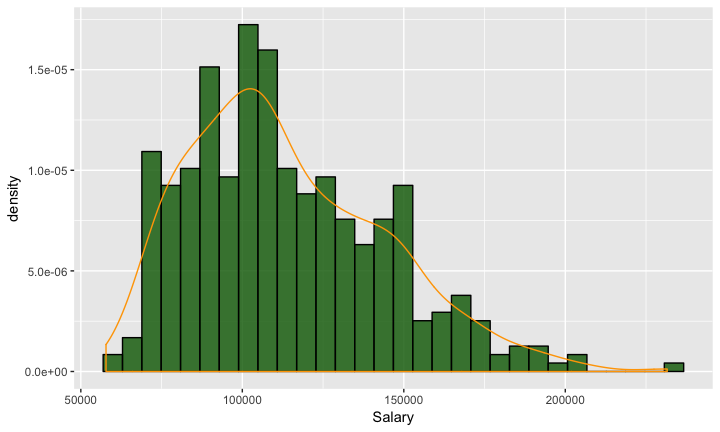
\includegraphics{Slides_files/figure-beamer/unnamed-chunk-7-1.pdf}

\end{block}

\begin{block}{AVERAGE SALARY PER RANK}

\begin{Shaded}
\begin{Highlighting}[]
\NormalTok{Mean_Salary <-}\StringTok{ }\NormalTok{prof_salary_tidy }\OperatorTok\StringTok{ }
\StringTok{  }\KeywordTok{group_by}\NormalTok{(Rank) }\OperatorTok\StringTok{ }
\StringTok{  }\KeywordTok{summarize}\NormalTok{(}\DataTypeTok{Mean_Salary=}\NormalTok{(}\KeywordTok{mean}\NormalTok{(Salary, }\DataTypeTok{na.rm =} \OtherTok{TRUE}\NormalTok{)))}
\NormalTok{Mean_Salary}
\end{Highlighting}
\end{Shaded}

\begin{verbatim}
## # A tibble: 3 x 2
##   Rank      Mean_Salary
##   <chr>           <dbl>
## 1 AssocProf      93876.
## 2 AsstProf       80776.
## 3 Prof          126772.
\end{verbatim}

\end{block}

\begin{block}{PUT THE NUMBERS IN A GRAPH}

\begin{Shaded}
\begin{Highlighting}[]
\NormalTok{Mean_Salary }\OperatorTok\StringTok{ }
\StringTok{  }\KeywordTok{ggplot}\NormalTok{(}\KeywordTok{aes}\NormalTok{(}\DataTypeTok{x=}\NormalTok{Rank, }\DataTypeTok{y=}\NormalTok{Mean_Salary,}\DataTypeTok{fill=}\NormalTok{Rank))}\OperatorTok{+}
\StringTok{  }\KeywordTok{geom_bar}\NormalTok{(}\DataTypeTok{stat=}\StringTok{"identity"}\NormalTok{, }\DataTypeTok{alpha=}\FloatTok{0.9}\NormalTok{, }\DataTypeTok{color=}\StringTok{"black"}\NormalTok{)}\OperatorTok{+}
\StringTok{  }\KeywordTok{labs}\NormalTok{(}\DataTypeTok{title =} \StringTok{"Mean Salary By Rank of Professors"}\NormalTok{,}
       \DataTypeTok{x =} \StringTok{"Rank"}\NormalTok{,}
       \DataTypeTok{y =} \StringTok{"Mean Salary"}\NormalTok{)}\OperatorTok{+}
\StringTok{  }\KeywordTok{theme}\NormalTok{(}\DataTypeTok{plot.title=}\KeywordTok{element_text}\NormalTok{(}\DataTypeTok{size=}\DecValTok{18}\NormalTok{, }\DataTypeTok{face=}\StringTok{"bold"}\NormalTok{, }\DataTypeTok{hjust =} \FloatTok{0.5}\NormalTok{),}
        \DataTypeTok{axis.text=}\KeywordTok{element_text}\NormalTok{(}\DataTypeTok{size=}\DecValTok{8}\NormalTok{),}
        \DataTypeTok{axis.title=}\KeywordTok{element_text}\NormalTok{(}\DataTypeTok{size=}\DecValTok{12}\NormalTok{))}\OperatorTok{+}
\StringTok{  }\KeywordTok{scale_fill_brewer}\NormalTok{(}\DataTypeTok{palette =} \StringTok{"Dark2"}\NormalTok{)}
\end{Highlighting}
\end{Shaded}

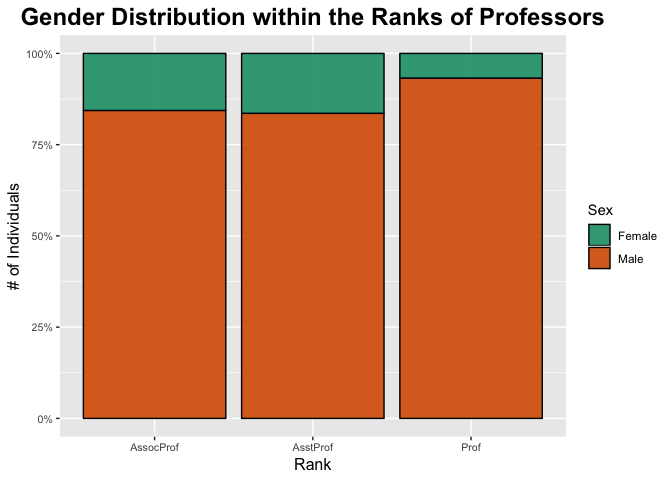
\includegraphics{Slides_files/figure-beamer/unnamed-chunk-9-1.pdf}
\#\#AVERAGE SALARY BY GENDER

\begin{Shaded}
\begin{Highlighting}[]
\NormalTok{Mean_Salary_Gender <-}\StringTok{ }\NormalTok{prof_salary_tidy }\OperatorTok\StringTok{ }
\StringTok{  }\KeywordTok{group_by}\NormalTok{(Sex) }\OperatorTok\StringTok{ }
\StringTok{  }\KeywordTok{summarize}\NormalTok{(}\DataTypeTok{Mean_Salary=}\NormalTok{(}\KeywordTok{mean}\NormalTok{(Salary, }\DataTypeTok{na.rm =} \OtherTok{TRUE}\NormalTok{)))}
\NormalTok{Mean_Salary_Gender}
\end{Highlighting}
\end{Shaded}

\begin{verbatim}
## # A tibble: 2 x 2
##   Sex    Mean_Salary
##   <chr>        <dbl>
## 1 Female     101002.
## 2 Male       115090.
\end{verbatim}

\end{block}

\begin{block}{PUT IT IN A GRAPH}

\begin{Shaded}
\begin{Highlighting}[]
\NormalTok{Mean_Salary_Gender }\OperatorTok\StringTok{ }
\StringTok{  }\KeywordTok{ggplot}\NormalTok{(}\KeywordTok{aes}\NormalTok{(}\DataTypeTok{x=}\NormalTok{Sex, }\DataTypeTok{y=}\NormalTok{Mean_Salary,}\DataTypeTok{fill=}\NormalTok{Sex))}\OperatorTok{+}
\StringTok{  }\KeywordTok{geom_bar}\NormalTok{(}\DataTypeTok{stat=}\StringTok{"identity"}\NormalTok{, }\DataTypeTok{alpha=}\FloatTok{0.9}\NormalTok{, }\DataTypeTok{color=}\StringTok{"black"}\NormalTok{)}\OperatorTok{+}
\StringTok{  }\KeywordTok{labs}\NormalTok{(}\DataTypeTok{title =} \StringTok{"Mean Salary By Gender"}\NormalTok{,}
       \DataTypeTok{x =} \StringTok{"Gender"}\NormalTok{,}
       \DataTypeTok{y =} \StringTok{"Mean Salary"}\NormalTok{)}\OperatorTok{+}
\StringTok{  }\KeywordTok{theme}\NormalTok{(}\DataTypeTok{plot.title=}\KeywordTok{element_text}\NormalTok{(}\DataTypeTok{size=}\DecValTok{18}\NormalTok{, }\DataTypeTok{face=}\StringTok{"bold"}\NormalTok{, }\DataTypeTok{hjust =} \FloatTok{0.5}\NormalTok{),}
        \DataTypeTok{axis.text=}\KeywordTok{element_text}\NormalTok{(}\DataTypeTok{size=}\DecValTok{8}\NormalTok{),}
        \DataTypeTok{axis.title=}\KeywordTok{element_text}\NormalTok{(}\DataTypeTok{size=}\DecValTok{12}\NormalTok{))}\OperatorTok{+}
\StringTok{  }\KeywordTok{scale_fill_brewer}\NormalTok{(}\DataTypeTok{palette =} \StringTok{"Dark2"}\NormalTok{)}
\end{Highlighting}
\end{Shaded}

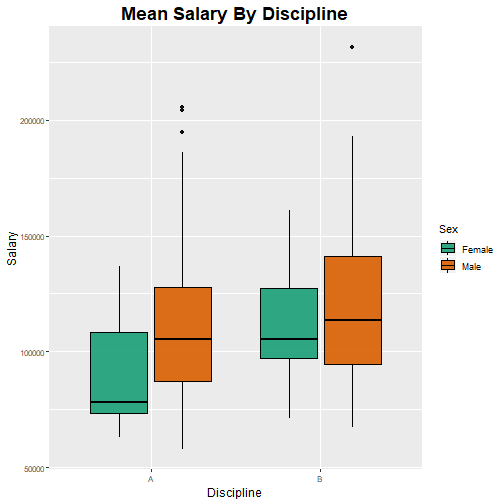
\includegraphics{Slides_files/figure-beamer/unnamed-chunk-11-1.pdf}
\#\#GENDER DISTRIBUTION

\begin{Shaded}
\begin{Highlighting}[]
\NormalTok{prof_salary_tidy }\OperatorTok\StringTok{ }
\StringTok{  }\KeywordTok{ggplot}\NormalTok{(}\KeywordTok{aes}\NormalTok{(}\DataTypeTok{x=}\NormalTok{Rank, }\DataTypeTok{fill=}\NormalTok{Sex))}\OperatorTok{+}
\StringTok{  }\KeywordTok{geom_bar}\NormalTok{(}\DataTypeTok{alpha=}\FloatTok{0.9}\NormalTok{, }\DataTypeTok{color=}\StringTok{"black"}\NormalTok{, }\DataTypeTok{position =} \KeywordTok{position_fill}\NormalTok{(), }\DataTypeTok{stat =} \StringTok{"count"}\NormalTok{)}\OperatorTok{+}
\StringTok{  }\KeywordTok{scale_y_continuous}\NormalTok{(}\DataTypeTok{labels =}\NormalTok{ scales}\OperatorTok{::}\NormalTok{percent)}\OperatorTok{+}
\StringTok{  }\KeywordTok{labs}\NormalTok{(}\DataTypeTok{title =} \StringTok{"Gender Distribution within the Ranks of Professors"}\NormalTok{,}
       \DataTypeTok{x =} \StringTok{"Rank"}\NormalTok{,}
       \DataTypeTok{y =} \StringTok{"# of Individuals"}\NormalTok{)}\OperatorTok{+}
\StringTok{  }\KeywordTok{theme}\NormalTok{(}\DataTypeTok{plot.title=}\KeywordTok{element_text}\NormalTok{(}\DataTypeTok{size=}\DecValTok{18}\NormalTok{, }\DataTypeTok{face=}\StringTok{"bold"}\NormalTok{, }\DataTypeTok{hjust =} \FloatTok{0.5}\NormalTok{),}
        \DataTypeTok{axis.text=}\KeywordTok{element_text}\NormalTok{(}\DataTypeTok{size=}\DecValTok{8}\NormalTok{),}
        \DataTypeTok{axis.title=}\KeywordTok{element_text}\NormalTok{(}\DataTypeTok{size=}\DecValTok{12}\NormalTok{))}\OperatorTok{+}
\StringTok{  }\KeywordTok{scale_fill_brewer}\NormalTok{(}\DataTypeTok{palette =} \StringTok{"Dark2"}\NormalTok{)}
\end{Highlighting}
\end{Shaded}

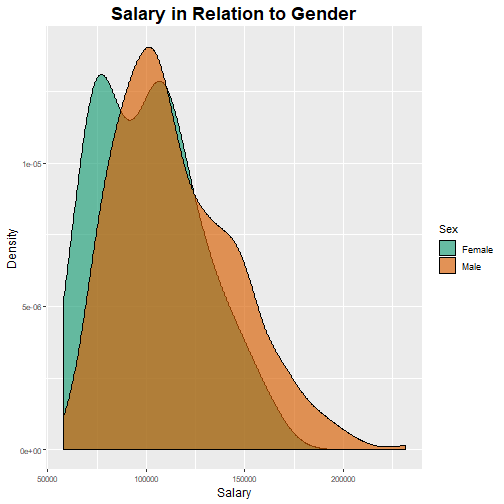
\includegraphics{Slides_files/figure-beamer/unnamed-chunk-12-1.pdf}

\end{block}

\end{frame}

\begin{frame}[fragile]

\begin{Shaded}
\begin{Highlighting}[]
\NormalTok{prof_salary_tidy }\OperatorTok\StringTok{ }
\StringTok{  }\KeywordTok{ggplot}\NormalTok{(}\KeywordTok{aes}\NormalTok{(}\DataTypeTok{x=}\NormalTok{Salary, }\DataTypeTok{fill=}\NormalTok{Sex))}\OperatorTok{+}
\StringTok{  }\KeywordTok{geom_density}\NormalTok{(}\DataTypeTok{alpha=}\FloatTok{0.65}\NormalTok{)}\OperatorTok{+}
\StringTok{  }\KeywordTok{labs}\NormalTok{(}\DataTypeTok{title =} \StringTok{"Salary in Relation to Gender"}\NormalTok{,}
       \DataTypeTok{x =} \StringTok{"Salary"}\NormalTok{,}
       \DataTypeTok{y =} \StringTok{"Density"}\NormalTok{)}\OperatorTok{+}
\StringTok{  }\KeywordTok{theme}\NormalTok{(}\DataTypeTok{plot.title=}\KeywordTok{element_text}\NormalTok{(}\DataTypeTok{size=}\DecValTok{18}\NormalTok{, }\DataTypeTok{face=}\StringTok{"bold"}\NormalTok{, }\DataTypeTok{hjust =} \FloatTok{0.5}\NormalTok{),}
        \DataTypeTok{axis.text=}\KeywordTok{element_text}\NormalTok{(}\DataTypeTok{size=}\DecValTok{8}\NormalTok{),}
        \DataTypeTok{axis.title=}\KeywordTok{element_text}\NormalTok{(}\DataTypeTok{size=}\DecValTok{12}\NormalTok{))}\OperatorTok{+}
\StringTok{  }\KeywordTok{scale_fill_brewer}\NormalTok{(}\DataTypeTok{palette =} \StringTok{"Dark2"}\NormalTok{)}
\end{Highlighting}
\end{Shaded}

\begin{block}{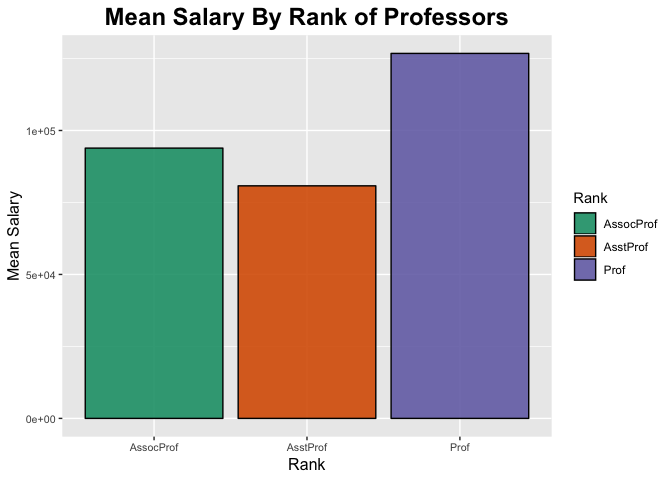
\includegraphics{Slides_files/figure-beamer/unnamed-chunk-13-1.pdf}}

\end{block}

\begin{block}{DISCIPLINES}

\begin{Shaded}
\begin{Highlighting}[]
\NormalTok{prof_salary_tidy }\OperatorTok\StringTok{ }
\StringTok{  }\KeywordTok{ggplot}\NormalTok{(}\KeywordTok{aes}\NormalTok{(}\DataTypeTok{x=}\NormalTok{Discipline, }\DataTypeTok{y=}\NormalTok{Salary, }\DataTypeTok{fill=}\NormalTok{Sex))}\OperatorTok{+}
\StringTok{  }\KeywordTok{geom_boxplot}\NormalTok{(}\DataTypeTok{alpha=}\FloatTok{0.9}\NormalTok{, }\DataTypeTok{color=}\StringTok{"black"}\NormalTok{)}\OperatorTok{+}
\StringTok{  }\KeywordTok{labs}\NormalTok{(}\DataTypeTok{title =} \StringTok{"Mean Salary By Discipline"}\NormalTok{,}
       \DataTypeTok{x =} \StringTok{"Discipline"}\NormalTok{,}
       \DataTypeTok{y =} \StringTok{"Salary"}\NormalTok{)}\OperatorTok{+}
\StringTok{  }\KeywordTok{theme}\NormalTok{(}\DataTypeTok{plot.title=}\KeywordTok{element_text}\NormalTok{(}\DataTypeTok{size=}\DecValTok{18}\NormalTok{, }\DataTypeTok{face=}\StringTok{"bold"}\NormalTok{, }\DataTypeTok{hjust =} \FloatTok{0.5}\NormalTok{),}
        \DataTypeTok{axis.text=}\KeywordTok{element_text}\NormalTok{(}\DataTypeTok{size=}\DecValTok{8}\NormalTok{),}
        \DataTypeTok{axis.title=}\KeywordTok{element_text}\NormalTok{(}\DataTypeTok{size=}\DecValTok{12}\NormalTok{))}\OperatorTok{+}
\StringTok{  }\KeywordTok{scale_fill_brewer}\NormalTok{(}\DataTypeTok{palette =} \StringTok{"Dark2"}\NormalTok{)}
\end{Highlighting}
\end{Shaded}

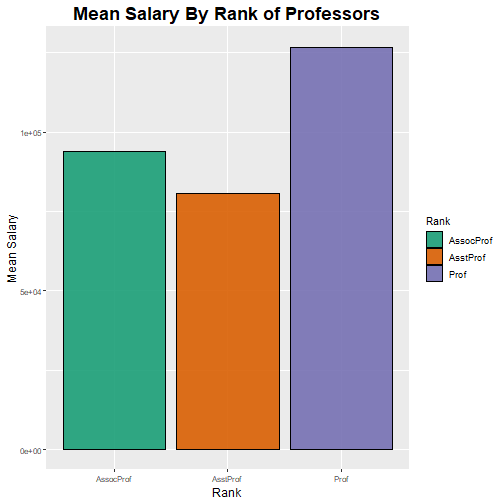
\includegraphics{Slides_files/figure-beamer/unnamed-chunk-14-1.pdf}

\end{block}

\begin{block}{YEARS SINCE RECEIVING A PHD}

\begin{Shaded}
\begin{Highlighting}[]
\NormalTok{prof_salary_tidy }\OperatorTok\StringTok{ }
\StringTok{  }\KeywordTok{ggplot}\NormalTok{(}\KeywordTok{aes}\NormalTok{(}\DataTypeTok{x=}\NormalTok{Yrs_since_PhD, }\DataTypeTok{y=}\NormalTok{Salary, }\DataTypeTok{color=}\NormalTok{Rank))}\OperatorTok{+}
\StringTok{  }\KeywordTok{geom_point}\NormalTok{(}\DataTypeTok{size=}\FloatTok{0.9}\NormalTok{)}\OperatorTok{+}
\StringTok{  }\KeywordTok{facet_wrap}\NormalTok{(}\OperatorTok{~}\NormalTok{Rank)}\OperatorTok{+}
\StringTok{  }\KeywordTok{geom_smooth}\NormalTok{(}\DataTypeTok{method=}\NormalTok{lm, }\DataTypeTok{se=}\OtherTok{TRUE}\NormalTok{)}\OperatorTok{+}
\StringTok{  }\KeywordTok{labs}\NormalTok{(}\DataTypeTok{title =} \StringTok{"Salary vs. Years Since PhD"}\NormalTok{,}
       \DataTypeTok{x =} \StringTok{"Years Since PhD"}\NormalTok{,}
       \DataTypeTok{y =} \StringTok{"Salary"}\NormalTok{)}\OperatorTok{+}
\StringTok{  }\KeywordTok{theme}\NormalTok{(}\DataTypeTok{plot.title=}\KeywordTok{element_text}\NormalTok{(}\DataTypeTok{size=}\DecValTok{18}\NormalTok{, }\DataTypeTok{face=}\StringTok{"bold"}\NormalTok{, }\DataTypeTok{hjust =} \FloatTok{0.5}\NormalTok{),}
        \DataTypeTok{axis.text=}\KeywordTok{element_text}\NormalTok{(}\DataTypeTok{size=}\DecValTok{8}\NormalTok{),}
        \DataTypeTok{axis.title=}\KeywordTok{element_text}\NormalTok{(}\DataTypeTok{size=}\DecValTok{12}\NormalTok{))}\OperatorTok{+}
\StringTok{  }\KeywordTok{scale_colour_brewer}\NormalTok{(}\DataTypeTok{palette =} \StringTok{"Dark2"}\NormalTok{)}
\end{Highlighting}
\end{Shaded}

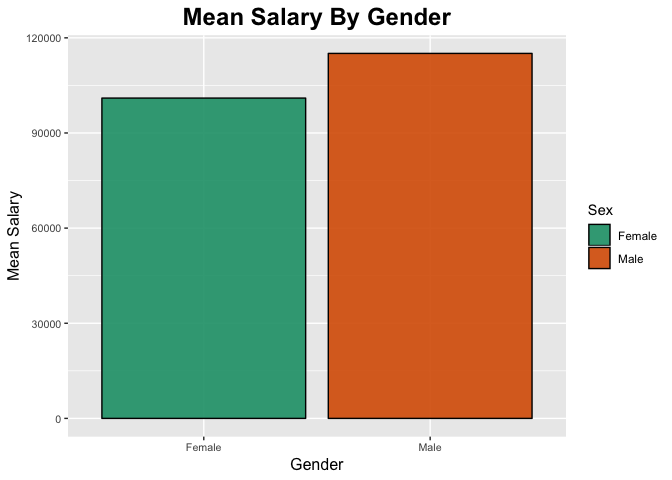
\includegraphics{Slides_files/figure-beamer/unnamed-chunk-15-1.pdf}

\end{block}

\begin{block}{YEARS SINCE SERVING}

\begin{Shaded}
\begin{Highlighting}[]
\NormalTok{prof_salary_tidy }\OperatorTok\StringTok{ }
\StringTok{  }\KeywordTok{ggplot}\NormalTok{(}\KeywordTok{aes}\NormalTok{(}\DataTypeTok{x=}\NormalTok{Yrs_service, }\DataTypeTok{y=}\NormalTok{Salary, }\DataTypeTok{color=}\NormalTok{Rank))}\OperatorTok{+}
\StringTok{  }\KeywordTok{geom_point}\NormalTok{(}\DataTypeTok{size=}\FloatTok{0.9}\NormalTok{)}\OperatorTok{+}
\StringTok{  }\KeywordTok{facet_wrap}\NormalTok{(}\OperatorTok{~}\NormalTok{Rank)}\OperatorTok{+}
\StringTok{  }\KeywordTok{geom_smooth}\NormalTok{(}\DataTypeTok{method=}\NormalTok{lm, }\DataTypeTok{se=}\OtherTok{TRUE}\NormalTok{)}\OperatorTok{+}
\StringTok{  }\KeywordTok{labs}\NormalTok{(}\DataTypeTok{title =} \StringTok{"Salary vs. Years Service"}\NormalTok{,}
       \DataTypeTok{x =} \StringTok{"Years Service"}\NormalTok{,}
       \DataTypeTok{y =} \StringTok{"Salary"}\NormalTok{)}\OperatorTok{+}
\StringTok{  }\KeywordTok{theme}\NormalTok{(}\DataTypeTok{plot.title=}\KeywordTok{element_text}\NormalTok{(}\DataTypeTok{size=}\DecValTok{18}\NormalTok{, }\DataTypeTok{face=}\StringTok{"bold"}\NormalTok{, }\DataTypeTok{hjust =} \FloatTok{0.5}\NormalTok{),}
        \DataTypeTok{axis.text=}\KeywordTok{element_text}\NormalTok{(}\DataTypeTok{size=}\DecValTok{8}\NormalTok{),}
        \DataTypeTok{axis.title=}\KeywordTok{element_text}\NormalTok{(}\DataTypeTok{size=}\DecValTok{12}\NormalTok{))}\OperatorTok{+}
\StringTok{  }\KeywordTok{scale_colour_brewer}\NormalTok{(}\DataTypeTok{palette =} \StringTok{"Dark2"}\NormalTok{)}
\end{Highlighting}
\end{Shaded}

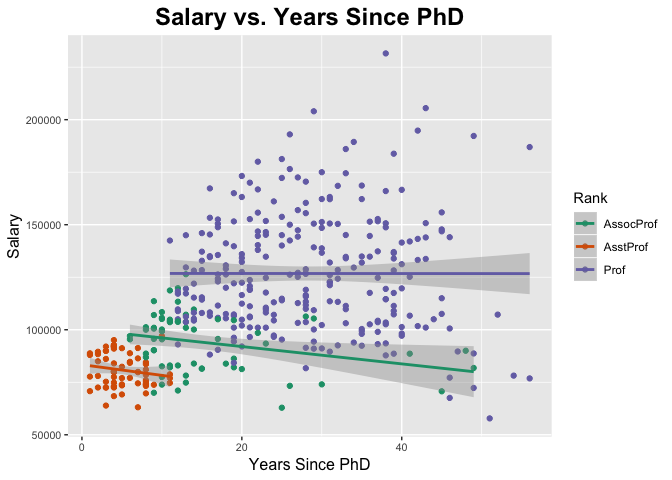
\includegraphics{Slides_files/figure-beamer/unnamed-chunk-16-1.pdf}

\end{block}

\begin{block}{CONCLUSIONS}

-There is a visible difference between salary of male professors and
female professors. However, the distribution of female and male
professors is more shocking.

\begin{itemize}
\item
  Assistant professors have the lowest average salary, while full
  professors have the highest average salary.
\item
  The longer a professor has been a PhD and serving, the higher salary
  s/he gets.
\end{itemize}

\end{block}

\end{frame}

\end{document}
